\documentclass{standalone}
\usepackage{tikz}
\usetikzlibrary{patterns, positioning}

\begin{document}
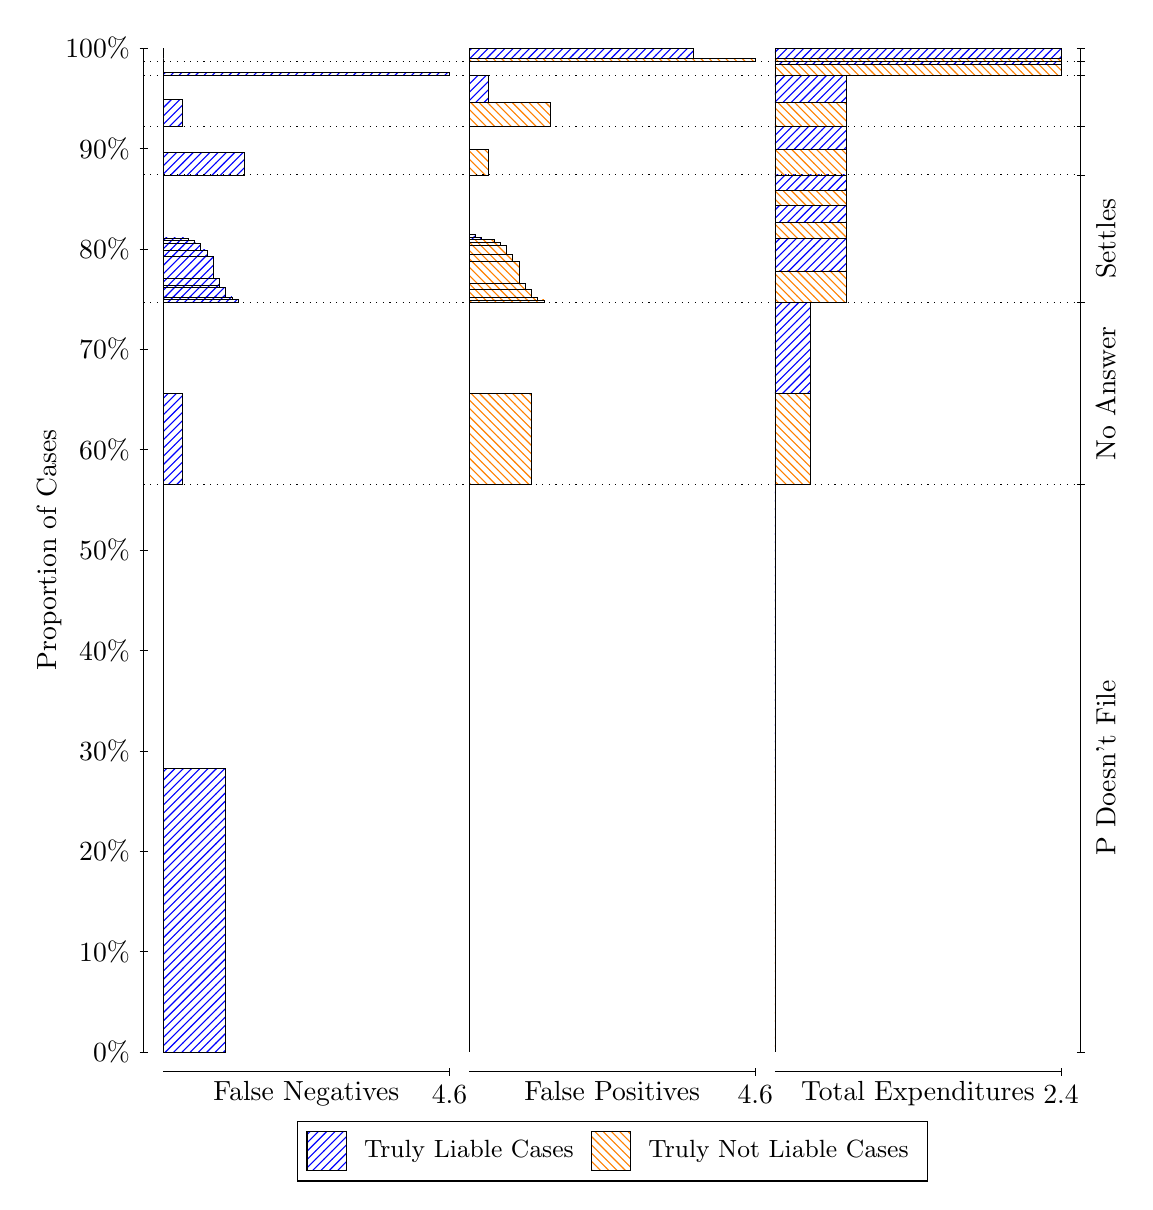
\begin{tikzpicture}
\draw[black, very thin] (1.5,1.75) -- (1.5,14.5);
\node[rotate=90, anchor=center] at (0.3, 8.125) {Proportion of Cases};
\draw[black, very thin] (1.45,1.75) -- (1.55,1.75);
\node[anchor=east] at (1.45, 1.75) {0\%};
\draw[black, very thin] (1.45,3.025) -- (1.55,3.025);
\node[anchor=east] at (1.45, 3.025) {10\%};
\draw[black, very thin] (1.45,4.3) -- (1.55,4.3);
\node[anchor=east] at (1.45, 4.3) {20\%};
\draw[black, very thin] (1.45,5.575) -- (1.55,5.575);
\node[anchor=east] at (1.45, 5.575) {30\%};
\draw[black, very thin] (1.45,6.85) -- (1.55,6.85);
\node[anchor=east] at (1.45, 6.85) {40\%};
\draw[black, very thin] (1.45,8.125) -- (1.55,8.125);
\node[anchor=east] at (1.45, 8.125) {50\%};
\draw[black, very thin] (1.45,9.4) -- (1.55,9.4);
\node[anchor=east] at (1.45, 9.4) {60\%};
\draw[black, very thin] (1.45,10.675) -- (1.55,10.675);
\node[anchor=east] at (1.45, 10.675) {70\%};
\draw[black, very thin] (1.45,11.95) -- (1.55,11.95);
\node[anchor=east] at (1.45, 11.95) {80\%};
\draw[black, very thin] (1.45,13.225) -- (1.55,13.225);
\node[anchor=east] at (1.45, 13.225) {90\%};
\draw[black, very thin] (1.45,14.5) -- (1.55,14.5);
\node[anchor=east] at (1.45, 14.5) {100\%};

\draw[black, very thin] (13.4,1.75) -- (13.4,14.5);
\draw[black, very thin] (13.35,1.75) -- (13.45,1.75);
\node[anchor=west] at (13.35, 1.75) {};
\draw[black, very thin] (13.35,8.961) -- (13.45,8.961);
\node[anchor=west] at (13.35, 8.961) {};
\draw[black, very thin] (13.35,11.266) -- (13.45,11.266);
\node[anchor=west] at (13.35, 11.266) {};
\draw[black, very thin] (13.35,12.89) -- (13.45,12.89);
\node[anchor=west] at (13.35, 12.89) {};
\draw[black, very thin] (13.35,13.505) -- (13.45,13.505);
\node[anchor=west] at (13.35, 13.505) {};
\draw[black, very thin] (13.35,14.152) -- (13.45,14.152);
\node[anchor=west] at (13.35, 14.152) {};
\draw[black, very thin] (13.35,14.333) -- (13.45,14.333);
\node[anchor=west] at (13.35, 14.333) {};
\draw[black, very thin] (13.35,14.5) -- (13.45,14.5);
\node[anchor=west] at (13.35, 14.5) {};

\draw[black, very thin, pattern color=blue, pattern=north east lines] (1.75,1.75) rectangle (2.5399,5.3555);
\draw[black, very thin, pattern color=orange, pattern=north west lines] (1.75,5.3555) rectangle (1.75,8.961);
\draw[black, very thin, pattern color=blue, pattern=north east lines] (1.75,8.961) rectangle (1.987,10.114);
\draw[black, very thin, pattern color=orange, pattern=north west lines] (1.75,10.114) rectangle (1.75,11.266);
\draw[black, very thin, pattern color=blue, pattern=north east lines] (1.75,11.266) rectangle (2.6978,11.304);
\draw[black, very thin, pattern color=blue, pattern=north east lines] (1.75,11.304) rectangle (2.6188,11.34);
\draw[black, very thin, pattern color=blue, pattern=north east lines] (1.75,11.34) rectangle (2.5399,11.464);
\draw[black, very thin, pattern color=blue, pattern=north east lines] (1.75,11.464) rectangle (2.4609,11.483);
\draw[black, very thin, pattern color=blue, pattern=north east lines] (1.75,11.483) rectangle (2.4609,11.57);
\draw[black, very thin, pattern color=blue, pattern=north east lines] (1.75,11.57) rectangle (2.3819,11.86);
\draw[black, very thin, pattern color=blue, pattern=north east lines] (1.75,11.86) rectangle (2.3029,11.935);
\draw[black, very thin, pattern color=blue, pattern=north east lines] (1.75,11.935) rectangle (2.2239,12.024);
\draw[black, very thin, pattern color=blue, pattern=north east lines] (1.75,12.024) rectangle (2.1449,12.056);
\draw[black, very thin, pattern color=blue, pattern=north east lines] (1.75,12.056) rectangle (2.0659,12.088);
\draw[black, very thin, pattern color=orange, pattern=north west lines] (1.75,12.088) rectangle (1.75,12.89);
\draw[black, very thin, pattern color=blue, pattern=north east lines] (1.75,12.89) rectangle (2.7768,13.178);
\draw[black, very thin, pattern color=orange, pattern=north west lines] (1.75,13.178) rectangle (1.75,13.505);
\draw[black, very thin, pattern color=blue, pattern=north east lines] (1.75,13.505) rectangle (1.987,13.845);
\draw[black, very thin, pattern color=orange, pattern=north west lines] (1.75,13.845) rectangle (1.75,14.152);
\draw[black, very thin, pattern color=blue, pattern=north east lines] (1.75,14.152) rectangle (5.3833,14.186);
\draw[black, very thin, pattern color=orange, pattern=north west lines] (1.75,14.186) rectangle (1.75,14.333);
\draw[black, very thin, pattern color=orange, pattern=north west lines] (1.75,14.333) rectangle (1.75,14.367);
\draw[black, very thin, pattern color=blue, pattern=north east lines] (1.75,14.367) rectangle (1.75,14.5);
\draw[black, very thin, pattern color=orange, pattern=north west lines] (5.6333,1.75) rectangle (5.6333,5.3556);
\draw[black, very thin, pattern color=blue, pattern=north east lines] (5.6333,5.3556) rectangle (5.6333,8.961);
\draw[black, very thin, pattern color=orange, pattern=north west lines] (5.6333,8.961) rectangle (6.4232,10.114);
\draw[black, very thin, pattern color=blue, pattern=north east lines] (5.6333,10.114) rectangle (5.6333,11.266);
\draw[black, very thin, pattern color=orange, pattern=north west lines] (5.6333,11.266) rectangle (6.5812,11.301);
\draw[black, very thin, pattern color=orange, pattern=north west lines] (5.6333,11.301) rectangle (6.5022,11.334);
\draw[black, very thin, pattern color=orange, pattern=north west lines] (5.6333,11.334) rectangle (6.4232,11.431);
\draw[black, very thin, pattern color=orange, pattern=north west lines] (5.6333,11.431) rectangle (6.3442,11.514);
\draw[black, very thin, pattern color=orange, pattern=north west lines] (5.6333,11.514) rectangle (6.2652,11.788);
\draw[black, very thin, pattern color=orange, pattern=north west lines] (5.6333,11.788) rectangle (6.1862,11.88);
\draw[black, very thin, pattern color=orange, pattern=north west lines] (5.6333,11.88) rectangle (6.1072,11.99);
\draw[black, very thin, pattern color=orange, pattern=north west lines] (5.6333,11.99) rectangle (6.0283,12.027);
\draw[black, very thin, pattern color=orange, pattern=north west lines] (5.6333,12.027) rectangle (5.9493,12.068);
\draw[black, very thin, pattern color=blue, pattern=north east lines] (5.6333,12.068) rectangle (5.7913,12.101);
\draw[black, very thin, pattern color=blue, pattern=north east lines] (5.6333,12.101) rectangle (5.7123,12.133);
\draw[black, very thin, pattern color=blue, pattern=north east lines] (5.6333,12.133) rectangle (5.6333,12.89);
\draw[black, very thin, pattern color=orange, pattern=north west lines] (5.6333,12.89) rectangle (5.8703,13.217);
\draw[black, very thin, pattern color=blue, pattern=north east lines] (5.6333,13.217) rectangle (5.6333,13.505);
\draw[black, very thin, pattern color=orange, pattern=north west lines] (5.6333,13.505) rectangle (6.6601,13.813);
\draw[black, very thin, pattern color=blue, pattern=north east lines] (5.6333,13.813) rectangle (5.8703,14.152);
\draw[black, very thin, pattern color=orange, pattern=north west lines] (5.6333,14.152) rectangle (5.6333,14.298);
\draw[black, very thin, pattern color=blue, pattern=north east lines] (5.6333,14.298) rectangle (5.6333,14.333);
\draw[black, very thin, pattern color=orange, pattern=north west lines] (5.6333,14.333) rectangle (9.2667,14.367);
\draw[black, very thin, pattern color=blue, pattern=north east lines] (5.6333,14.367) rectangle (8.4768,14.5);
\draw[black, very thin, pattern color=orange, pattern=north west lines] (9.5167,1.75) rectangle (9.5167,5.3556);
\draw[black, very thin, pattern color=blue, pattern=north east lines] (9.5167,5.3556) rectangle (9.5167,8.961);
\draw[black, very thin, pattern color=orange, pattern=north west lines] (9.5167,8.961) rectangle (9.9708,10.114);
\draw[black, very thin, pattern color=blue, pattern=north east lines] (9.5167,10.114) rectangle (9.9708,11.266);
\draw[black, very thin, pattern color=orange, pattern=north west lines] (9.5167,11.266) rectangle (10.425,11.669);
\draw[black, very thin, pattern color=blue, pattern=north east lines] (9.5167,11.669) rectangle (10.425,12.08);
\draw[black, very thin, pattern color=orange, pattern=north west lines] (9.5167,12.08) rectangle (10.425,12.288);
\draw[black, very thin, pattern color=blue, pattern=north east lines] (9.5167,12.288) rectangle (10.425,12.505);
\draw[black, very thin, pattern color=orange, pattern=north west lines] (9.5167,12.505) rectangle (10.425,12.695);
\draw[black, very thin, pattern color=blue, pattern=north east lines] (9.5167,12.695) rectangle (10.425,12.89);
\draw[black, very thin, pattern color=orange, pattern=north west lines] (9.5167,12.89) rectangle (10.425,13.217);
\draw[black, very thin, pattern color=blue, pattern=north east lines] (9.5167,13.217) rectangle (10.425,13.505);
\draw[black, very thin, pattern color=orange, pattern=north west lines] (9.5167,13.505) rectangle (10.425,13.813);
\draw[black, very thin, pattern color=blue, pattern=north east lines] (9.5167,13.813) rectangle (10.425,14.152);
\draw[black, very thin, pattern color=orange, pattern=north west lines] (9.5167,14.152) rectangle (13.15,14.298);
\draw[black, very thin, pattern color=blue, pattern=north east lines] (9.5167,14.298) rectangle (13.15,14.333);
\draw[black, very thin, pattern color=orange, pattern=north west lines] (9.5167,14.333) rectangle (13.15,14.367);
\draw[black, very thin, pattern color=blue, pattern=north east lines] (9.5167,14.367) rectangle (13.15,14.5);
\draw[black, dotted] (1.5,8.961) -- (13.4,8.961);
\draw[black, dotted] (1.5,11.266) -- (13.4,11.266);
\draw[black, dotted] (1.5,12.89) -- (13.4,12.89);
\draw[black, dotted] (1.5,13.505) -- (13.4,13.505);
\draw[black, dotted] (1.5,14.152) -- (13.4,14.152);
\draw[black, dotted] (1.5,14.333) -- (13.4,14.333);
\draw[black, very thin] (1.75,1.5) -- (5.3833,1.5);
\node[anchor=north] at (3.5667, 1.5) {False Negatives};
\draw[black, very thin] (5.3833,1.45) -- (5.3833,1.55);
\node[anchor=north] at (5.3833, 1.45) {4.6};

\draw[black, very thin] (5.6333,1.5) -- (9.2667,1.5);
\node[anchor=north] at (7.45, 1.5) {False Positives};
\draw[black, very thin] (9.2667,1.45) -- (9.2667,1.55);
\node[anchor=north] at (9.2667, 1.45) {4.6};

\draw[black, very thin] (9.5167,1.5) -- (13.15,1.5);
\node[anchor=north] at (11.333, 1.5) {Total Expenditures};
\draw[black, very thin] (13.15,1.45) -- (13.15,1.55);
\node[anchor=north] at (13.15, 1.45) {2.4};

\node[black, centered, rotate=90] at (13.72, 5.3555) {P Doesn't File};
\node[black, centered, rotate=90] at (13.72, 10.114) {No Answer};
\node[black, centered, rotate=90] at (13.72, 12.078) {Settles};





\draw (7.449999999999999,1.5) node[draw=none] (baseCoordinate) {};
\begin{scope}[align=center]
        \matrix[scale=0.5, draw=black, below=0.5cm of baseCoordinate, nodes={draw}, column sep=0.1cm]{
            \node[rectangle, draw, minimum width=0.5cm, minimum height=0.5cm, pattern=north east lines, pattern color=blue] {}; &
            \node[draw=none, font=\small] (B) {Truly Liable Cases}; &
            \node[rectangle, draw, minimum width=0.5cm, minimum height=0.5cm, pattern=north west lines, pattern color=orange] {}; &
            \node[draw=none, font=\small] (B) {Truly Not Liable Cases}; \\
            };
\end{scope}

\end{tikzpicture}
\end{document}